% ============================================================
%  FlowKit 캡스톤 보고서 — 2단 학술논문 형식
%  컴파일: XeLaTeX 또는 LuaLaTeX (kotex 패키지 필요)
%  명령: xelatex 최종보고서_논문형.tex
% ============================================================

\documentclass[10pt, a4paper]{article}

% ── 언어 / 인코딩 ──────────────────────────────────────────
\usepackage{kotex}          % 한글 지원 (XeLaTeX/LuaLaTeX 권장)

% ── 레이아웃 ───────────────────────────────────────────────
\usepackage[
  top=25mm, bottom=25mm,
  left=20mm, right=20mm,
  columnsep=7mm
]{geometry}
\usepackage{multicol}       % 2단 레이아웃

% ── 그림 / 표 ──────────────────────────────────────────────
\usepackage{graphicx}
\usepackage{booktabs}
\usepackage{tabularx}
\usepackage{array}
\usepackage{caption}
\usepackage{float}

% ── 글꼴 / 타이포그래피 ────────────────────────────────────
\usepackage{setspace}
\usepackage{microtype}
\captionsetup{font=small, labelfont=bf, skip=4pt}

% ── 섹션 제목 스타일 ───────────────────────────────────────
\usepackage{titlesec}
\titleformat{\section}[block]
  {\normalfont\normalsize\bfseries\centering}{}{0pt}{}
\titleformat{\subsection}[block]
  {\normalfont\normalsize\bfseries}{}{0pt}{}
\titleformat{\subsubsection}[block]
  {\normalfont\small\bfseries}{}{0pt}{}
\titlespacing*{\section}{0pt}{8pt}{4pt}
\titlespacing*{\subsection}{0pt}{6pt}{3pt}
\titlespacing*{\subsubsection}{0pt}{4pt}{2pt}

% ── 기타 ───────────────────────────────────────────────────
\usepackage{hyperref}
\hypersetup{colorlinks=true, linkcolor=black, citecolor=black, urlcolor=blue}
\usepackage{lipsum}
\pagestyle{plain}

% ============================================================
%  문서 시작
% ============================================================
\begin{document}

% ── 표지 (1단, 전체 폭) ─────────────────────────────────────
\begin{center}
  {\large\bfseries FlowKit: 사용자 주도형 AI 대화 맥락 관리 서비스}\\[10pt]

  {\normalsize
    류건호\textsuperscript{*},\ 이호열\textsuperscript{*},\ 홍준서\textsuperscript{*},\ 조창현\textsuperscript{*}
  }\\[4pt]

  {\small
    \textsuperscript{*}서울과학기술대학교 인공지능응용학과\\[4pt]
    \textbf{지도교수:} 서경원 교수 (서울과학기술대학교 인공지능응용학과)\\[2pt]
    서울과학기술대학교\ |\ 2026년 6월
  }
\end{center}

\vspace{4pt}\hrule\vspace{6pt}

% ── 요약 (1단) ───────────────────────────────────────────────
\noindent\textbf{요\ 약}\ \ 생성형 AI 챗봇이 다양한 장기 작업에 광범위하게 활용되면서, 긴 다중 턴 대화에서 사용자가
AI의 맥락 처리를 직접 제어하기 어렵다는 문제가 대두되고 있다. 기존 챗봇은 이전 대화를 시간순으로 자동 누적하여
후속 응답에 반영하지만, 이 방식은 폐기된 아이디어나 읽지 않은 응답이 맥락으로 지속 반영되는 한계를 지닌다. 본
연구에서는 이러한 문제를 해결하기 위해 FlowKit을 제안한다. FlowKit은 대화를 메시지 블록(Message Block) 단위로
구조화하여, 사용자가 필요한 블록만 선택하고 자연어 지시로 Context를 정제한 뒤 후속 질문 또는 브랜치 생성에 적용할
수 있는 사용자 주도형 Context 관리 서비스이다. 캡스톤디자인(1)에서는 문제 정의, AS-IS/TO-BE 분석, 선행연구 조사,
UI/UX 프로토타입 설계, 시스템 구조 설계, 요구사항정의서 작성, 평가 계획 수립을 완료하였으며, 캡스톤디자인(2)에서
실제 구현 및 검증을 수행할 예정이다.

\vspace{4pt}
\noindent\textbf{핵심어:} Context Engineering, 메시지 블록 선택, 대화 브랜치, 사용자 주도형 맥락 관리, HCI

\vspace{6pt}\hrule\vspace{8pt}

% ============================================================
%  2단 본문 시작
% ============================================================
\begin{multicols}{2}

% ─────────────────────────────────────────────────────────
\section*{Ⅰ. 서론}
% ─────────────────────────────────────────────────────────

\subsection*{1. 연구 배경 및 필요성}

ChatGPT, Claude, Gemini 등 생성형 AI 챗봇은 학습, 문서 작성, 정보 정리, 아이디어 기획 등 다양한 작업에 광범위하게 활용되고 있다. 사용자는 단순한 질의응답을 넘어 여러 차례의 대화를 거치며 개념을 학습하거나, 보고서 초안을 수정하거나, 여러 아이디어를 비교·발전시키는 방식으로 AI 챗봇을 사용한다. 이에 따라 AI가 이전 대화 중 어떤 내용을 기억하고 후속 응답에 반영하는지가 중요한 문제가 되고 있다.

기존 AI 챗봇은 일반적으로 사용자 입력과 AI 응답을 시간순 대화 기록으로 누적하고, 후속 질문이 들어오면 이전 대화의 상당 부분을 맥락(Context)으로 활용한다. 이 방식은 짧은 대화에서는 편리하지만, 대화가 길어질수록 사용자가 실제로 읽거나 수용한 내용과 AI가 후속 응답에 반영하는 내용 사이에 차이가 발생할 수 있다.

따라서 다중 턴 대화 환경에서는 AI가 더 많은 내용을 자동으로 기억하는 것보다, 사용자가 필요한 맥락을 선택하고 불필요한 맥락을 제외할 수 있는 구조가 필요하다.

\subsection*{2. 기존 AI 챗봇의 한계}

ChatGPT, Claude, Gemini 등 현재 주요 채팅 서비스에서는 AI가 어떤 Context를 기억하고 활용하는지 사용자가 직접 확인하거나 조정하기 어렵다. 대화 전체가 하나의 선형 기록으로 누적되기 때문에 세밀한 제어가 어렵다.

또한 일부 서비스가 대화 분기 기능을 제공하더라도, 특정 시점까지의 전체 대화를 기준으로 분기하는 방식에 가깝다. 이 경우 사용자는 이전 대화 중 필요한 일부 의미 단위만 선택하여 새로운 대화 흐름으로 이어가기 어렵다.

ChatGPT의 Memory 기능이나 Claude의 Projects 기능은 AI가 특정 정보를 장기적으로 기억할 수 있게 한다는 점에서 맥락 관리의 필요성을 인식한 시도이다. 그러나 이들은 AI가 자동으로 요약·저장하는 방식에 기반하며, 사용자가 개별 메시지 블록 단위로 어떤 내용을 다음 응답에 반영할지 직접 선택·정제하는 구조가 아니다. 사용자는 어떤 대화 내용이 기억되는지 실시간으로 확인하거나, 특정 대화 단위만 선택하여 다음 응답의 맥락으로 지정하는 세밀한 제어를 하기 어렵다. FlowKit은 이러한 기존 서비스들과 달리, 맥락 구성의 주도권 자체를 사용자에게 명시적으로 이전하는 방식을 택한다.

선행연구 역시 긴 Context를 단순히 많이 제공하는 방식의 한계를 지적한다. Liu et al.~\cite{liu2024} 은 긴 Context 내부에서 관련 정보의 위치에 따라 LLM의 활용 성능이 달라질 수 있음을 보였으며, Laban et al.~\cite{laban2025} 은 다중 턴 대화에서 모델이 초기 가정이나 이전 응답에 과도하게 의존할 수 있음을 지적하였다.

\subsection*{3. 연구 목적 및 범위}

FlowKit은 기존 AI 챗봇의 선형적 Context 누적 문제를 해결하기 위해 제안된 사용자 주도형 AI 대화 맥락 관리 서비스이다. FlowKit은 대화를 메시지 블록(Message Block) 단위로 나누고, 사용자가 필요한 블록만 선택하여 다음 대화의 Context로 활용할 수 있게 한다.

FlowKit의 설계 방향은 Context를 사용자가 조작 가능한 상호작용 객체로 보아야 한다는 Mixed-Initiative Context 연구~\cite{li2026}와도 연결된다. FlowKit은 LLM 모델 자체를 새로 학습시키는 프로젝트가 아니라, 사용자 인터페이스 차원에서 Context를 명시화하고, 선택·편집·분기할 수 있도록 하는 HCI 기반 Context 관리 서비스이다.

\subsection*{4. 보고서 구성}

본 보고서는 다음과 같이 구성된다. Ⅱ장에서는 FlowKit의 설계 근거가 되는 선행연구를 기술한다. Ⅲ장에서는 시스템 설계를 상세히 기술한다. Ⅳ장에서는 연구 요약, 활용 분야, 향후 확장 가능성을 제시한다.

% ─────────────────────────────────────────────────────────
\section*{Ⅱ. 관련 연구}
% ─────────────────────────────────────────────────────────

FlowKit의 설계는 세 가지 연구 축에 기반한다. 첫째, 대화 기록 전체를 그대로 Context로 사용하는 방식이 실제로 문제를 야기한다는 실증 근거, 둘째, Context를 사용자가 직접 선택·편집할 수 있는 상호작용 객체로 재정의한 이론적 기반, 셋째, 선형 대화를 분기 가능한 구조로 관리하는 대화 버전 관리 연구가 그것이다. 이 절에서는 세 축의 논문들을 흐름에 따라 검토하며, 각 연구가 FlowKit의 어느 문제의식 또는 설계 결정과 연결되는지를 설명한다.

\subsection*{1. 선형 누적 Context의 실증적 한계}

FlowKit의 출발점은 ``긴 대화를 그대로 Context로 넣는 것이 항상 최선은 아니다''라는 주장이다. 이를 뒷받침하는 가장 신뢰할 수 있는 근거는 Liu et al.~\cite{liu2024}과 Laban et al.~\cite{laban2025}이 각각 다른 차원에서 제시한 두 가지 실증 결과다.

Liu et al.~\cite{liu2024}은 긴 Context를 처리할 수 있는 LLM이라도, 관련 정보가 Context의 중간 부분에 위치할 때 성능이 저하되는 ``Lost in the Middle'' 현상을 실험적으로 보고하였다. 이 연구는 context window가 충분히 크더라도 입력된 정보가 균등하게 반영되지 않을 수 있음을 입증한 peer-reviewed 논문(TACL 2024)으로, 긴 대화 기록 전체를 Context로 제공하는 방식이 항상 최선이 아님을 정량적으로 보여준다.

Laban et al.~\cite{laban2025}은 여기서 한 단계 더 나아간다. 동일한 요구사항을 단일 턴에 제공받는 경우와 여러 턴에 걸쳐 점진적으로 드러나는 경우를 비교하면, 다중 턴 대화에서 모델이 초기 가정이나 이전 응답에 과도하게 의존하며 응답 품질이 저하될 수 있음을 보였다. Liu et al.이 ``Context 내부의 위치 문제''를 다루었다면, Laban et al.은 ``대화가 누적되는 시간 축의 문제''를 다루었다.

두 연구는 서로 다른 차원에서 동일한 방향을 가리킨다. FlowKit이 사용자가 필요한 블록만 선택하여 불필요한 맥락 노이즈를 제거하는 구조를 택한 것은 이 실증 결과에 직접적으로 반응한 설계 결정이다.

\subsection*{2. Context를 조작 가능한 객체로 — 핵심 이론 기반}

FlowKit의 설계 원리를 가장 직접적으로 이론화한 연구는 Li et al.~\cite{li2026}의 Mixed-Initiative Context이다. 이 연구는 Human-AI Collaboration 환경에서 Context를 숨겨진 모델 입력이 아닌, 사용자가 직접 포함·제외·수정·재조직할 수 있는 명시적 상호작용 객체(interactive artifact)로 재정의한다. AI는 브랜치 제안이나 패턴 추출 등을 통해 사용자를 보조하되, Context의 최종 구성 권한은 사용자에게 있어야 한다는 것이 이 연구의 핵심 주장이다.

이 개념은 FlowKit의 각 기능과 거의 일대일로 대응된다. 메시지 블록 선택은 Context unit의 포함·제외에, Context 편집 패널은 Context를 가시적·조작 가능하게 만드는 인터페이스에, 자연어 편집 지시는 사용자 주도 Context 재조직에, 정제 결과 미리보기 후 적용은 AI 제안을 사용자가 승인하는 Mixed-Initiative 구조에 각각 대응한다.

Human-in-the-loop 설계의 필요성은 Tso et al.~\cite{tso2026}의 연구가 보조적으로 지지한다. 이 연구는 최신 LLM도 제약 조건이 포함된 작업에서 사용자 의도를 안정적으로 만족하지 못하는 경우가 있음을 벤치마크로 보였다. FlowKit에서 AI가 생성한 정제 Context를 자동으로 반영하지 않고, 사용자가 미리보기로 확인·승인한 뒤에만 적용하는 단계를 설계한 근거가 여기서도 확인된다.

\subsection*{3. 원본 로그와 활성 Context의 분리 — 시스템 구조 참고}

이론적 원리를 구현하려면 내부 데이터 구조도 이를 뒷받침해야 한다. Packer et al.~\cite{packer2023}의 MemGPT는 운영체제의 메모리 계층 구조를 LLM에 적용하여, 전체 대화 로그(long-term storage)와 LLM에 실제 전달되는 맥락(in-context storage)을 분리 관리하는 virtual context management 구조를 제안하였다.

FlowKit 역시 Raw Conversation(원본 대화 로그)과 Active Prompt(다음 LLM 응답에 실제 반영되는 맥락)를 분리하는 구조를 채택한다. 다만 MemGPT가 시스템이 자동으로 메모리를 관리하는 agent-managed 구조라면, FlowKit은 사용자가 직접 어떤 블록을 Active Prompt에 포함할지 결정하는 user-managed 구조라는 것이 핵심 차이다.

\subsection*{4. 대화 버전 관리와 선택형 브랜치}

Context를 사용자가 선택·정제한다면, 그 Context를 기반으로 새로운 대화 흐름을 분기하는 것도 자연스러운 확장이다. Nanjundappa and Maaheshwari~\cite{nanjundappa2025}의 ContextBranch는 LLM 대화에 소프트웨어 버전 관리 개념을 적용하여, checkpoint, branch, switch, inject라는 네 가지 기본 연산을 제안하였다. 이 연구는 선형 대화가 누적될수록 context pollution이 발생하며, 사용자가 새 채팅을 시작하면 오히려 유용한 맥락까지 잃는다는 딜레마를 구조적으로 지적한다.

FlowKit의 선택 Context 기반 브랜치 생성은 이 연구에서 직접적인 설계 근거를 가져온다. ContextBranch가 특정 checkpoint까지의 전체 대화를 기준으로 브랜치를 구성하는 방식이었다면, FlowKit은 사용자가 선택한 의미 단위의 메시지 블록만을 기반으로 새로운 대화 흐름을 생성한다. 또한 ContextBranch가 탐색적 프로그래밍 시나리오에 집중하였다면, FlowKit은 학습, 문서 작성, 정보 정리 등 일상적인 장기 대화 전반으로 적용 범위를 확장한다.

이상 네 편의 연구는 각기 다른 층위에서 FlowKit을 지지한다. Liu et al.과 Laban et al.은 문제의 존재를 실증하고, Li et al.은 핵심 설계 원리를 이론화하며, Packer et al.은 내부 데이터 구조의 선례를 제공하고, Nanjundappa et al.은 브랜치 기능의 구조적 기반이 된다. FlowKit은 이 연구들이 각각 분리되어 다루었던 문제의식과 해법을 하나의 사용자 인터페이스로 통합하고자 하는 시도이다.

% ─────────────────────────────────────────────────────────
\section*{Ⅲ. 시스템 설계}
% ─────────────────────────────────────────────────────────

\subsection*{1. 서비스 개요 및 AS-IS / TO-BE 분석}

기존 AI 챗봇의 대화 구조는 선형적이다. 사용자의 질문과 AI의 응답이 시간순으로 쌓이고, 후속 질문은 이전 대화 기록을 기반으로 처리된다. FlowKit은 이러한 문제를 해결하기 위해 대화 기록을 선택 가능한 Message Block 단위로 구조화한다.

\begin{table}[H]
\centering
\caption{일반 챗봇과 FlowKit의 구조 비교}
\label{tab:comparison}
\small
\begin{tabularx}{\columnwidth}{@{} l X X @{}}
\toprule
\textbf{구분} & \textbf{일반 챗봇} & \textbf{FlowKit} \\
\midrule
이전 대화 처리    & 전체 자동 반영    & 필요 블록 선택      \\
Context 가시성 & 확인 어려움      & 패널에서 확인 가능   \\
긴 응답 처리     & 전체 그대로 누적   & 요약·삭제·재작성   \\
대화 분기       & 시점 기준 분기    & 선택 Context 기준  \\
사용자 제어권     & 낮음           & 높음             \\
\bottomrule
\end{tabularx}
\end{table}

\subsection*{2. 사용자 사용 흐름}

FlowKit의 기본 사용 흐름은 다음과 같다. 사용자는 ① 질문 입력 → ② 필요한 메시지 블록 선택 → ③ Context 편집 패널 확인 → ④ 자연어 편집 지시 입력 → ⑤ 정제 Context 미리보기 확인 → ⑥ Context 적용 또는 브랜치 생성 순서로 서비스를 조작한다.

\begin{table}[H]
\centering
\caption{FlowKit 사용자 사용 흐름}
\label{tab:flow}
\small
\begin{tabularx}{\columnwidth}{@{} c X X @{}}
\toprule
\textbf{단계} & \textbf{사용자 행동} & \textbf{시스템 처리} \\
\midrule
1 & 질문 입력          & AI 응답 생성          \\
2 & 메시지 블록 선택      & Context 후보로 저장    \\
3 & 편집 패널 확인       & 선택 블록 목록 표시      \\
4 & 자연어 편집 지시      & Context 요약·재작성    \\
5 & 미리보기 확인        & 적용 전 결과 표시       \\
6 & Context 적용/분기   & 후속 응답 또는 브랜치 생성  \\
\bottomrule
\end{tabularx}
\end{table}

\subsection*{3. 핵심 기능 정의}

FlowKit의 핵심 기능은 기본 채팅 및 Message Block 구조, Context 편집 패널, AI 기반 Context 정제, Context 적용, 선택형 브랜치 생성, 메시지 수정 및 버전 관리로 구성된다.

\begin{table}[H]
\centering
\caption{FlowKit 핵심 기능 우선순위}
\label{tab:features}
\small
\begin{tabularx}{\columnwidth}{@{} c X @{}}
\toprule
\textbf{순위} & \textbf{기능} \\
\midrule
1 & 기본 채팅 및 Message Block 구조 \\
2 & Context 편집 패널 \\
3 & AI 기반 Context 정제 \\
4 & Context 적용 \\
5 & 선택형 브랜치 생성 \\
6 & 메시지 수정 및 버전 관리 \\
7 & Self-Correction (고도화) \\
8 & RAG / 외부 문서 연동 (고도화) \\
\bottomrule
\end{tabularx}
\end{table}

\subsection*{4. UI/UX 프로토타입 설계}

FlowKit의 UI/UX는 좌측 사이드바, 중앙 채팅 영역, 우측 Context 편집 패널의 3단 구조를 기본으로 한다. 좌측 사이드바는 전체 대화와 브랜치를 관리한다. 중앙 채팅 영역은 Message Block 단위로 메시지를 표시한다. 우측 Context 편집 패널은 선택된 블록 목록, 빠른 편집 버튼, AI 편집 지시 입력창, 정제된 Context 미리보기, Context 적용 버튼, 브랜치 생성 버튼을 제공한다.

\begin{figure}[H]
  \centering
  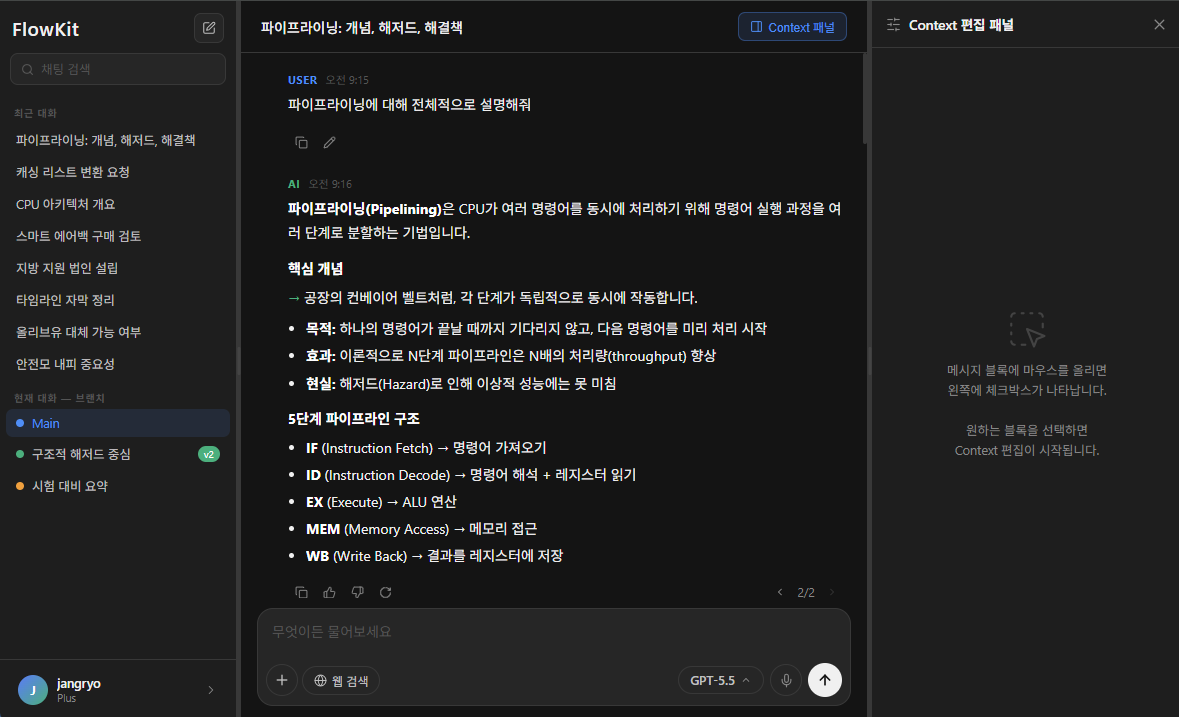
\includegraphics[width=\columnwidth]{images/그림1.png}
  \caption{FlowKit 전체 화면 — 좌측 사이드바, 중앙 메시지 블록 기반 채팅 영역, 우측 Context 편집 패널이 함께 표시된 전체 서비스 화면}
  \label{fig:fig1}
\end{figure}

\begin{figure}[H]
  \centering
  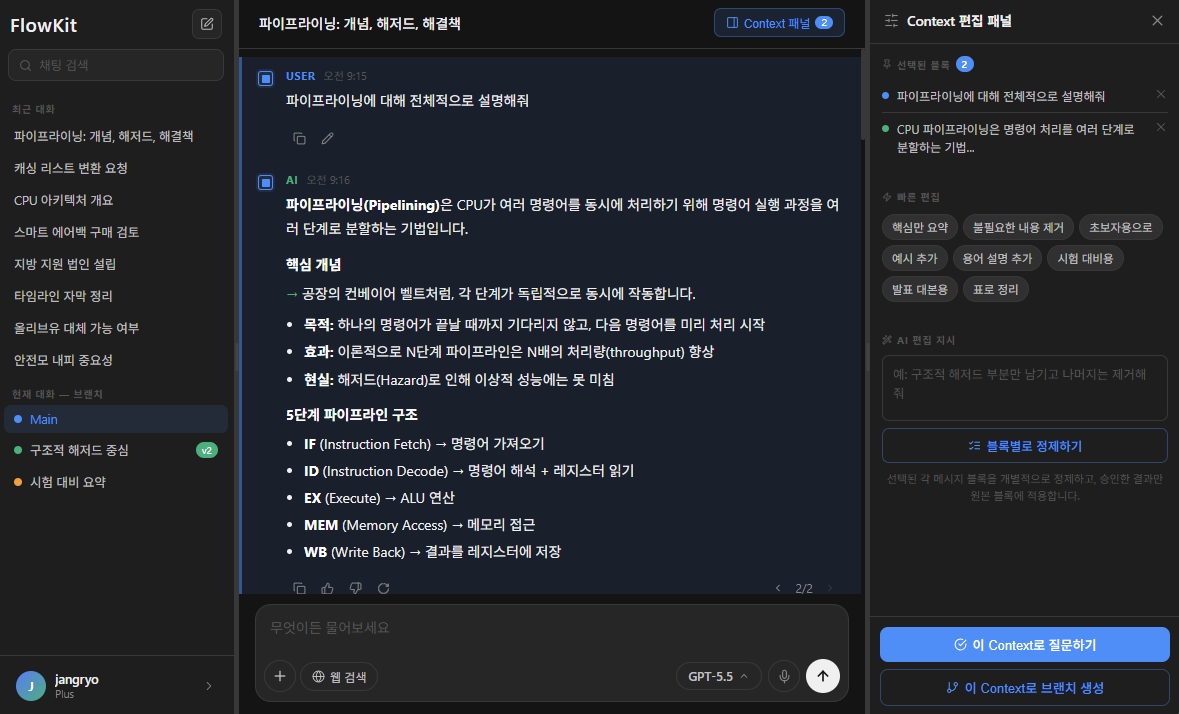
\includegraphics[width=\columnwidth]{images/그림2.png}
  \caption{메시지 블록 선택 및 Context 편집 패널 활성화 화면}
  \label{fig:fig2}
\end{figure}

\begin{figure}[H]
  \centering
  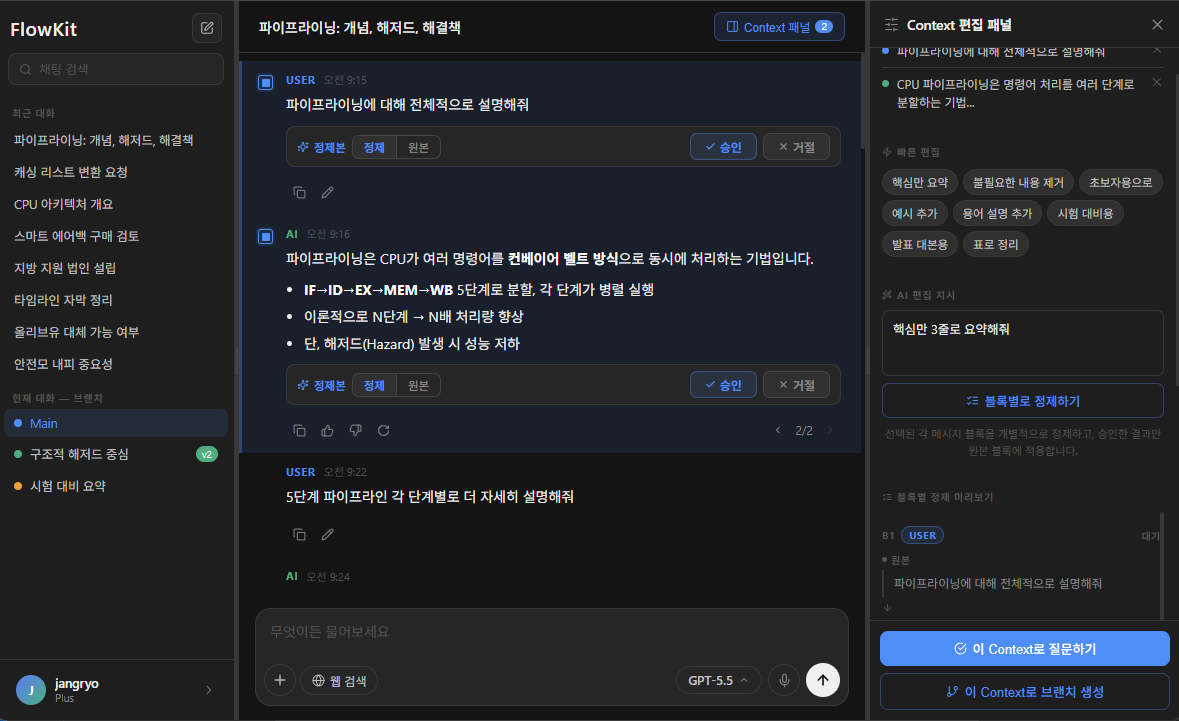
\includegraphics[width=\columnwidth]{images/그림3.png}
  \caption{블록별 정제 및 인라인 승인/거절 화면}
  \label{fig:fig3}
\end{figure}

\begin{figure}[H]
  \centering
  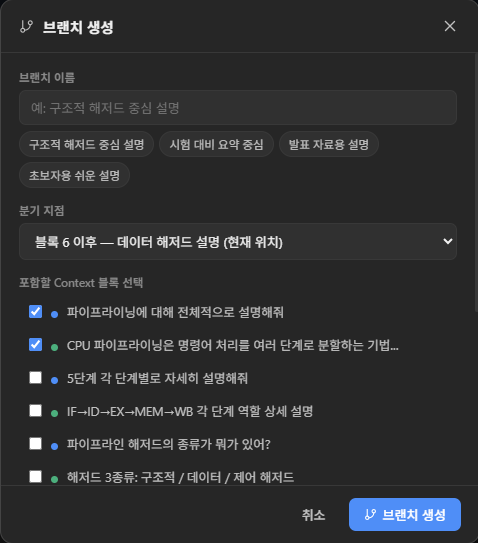
\includegraphics[width=\columnwidth]{images/그림4-1.png}
  \caption{선택 Context 기반 브랜치 생성 모달}
  \label{fig:fig4a}
\end{figure}

\begin{figure}[H]
  \centering
  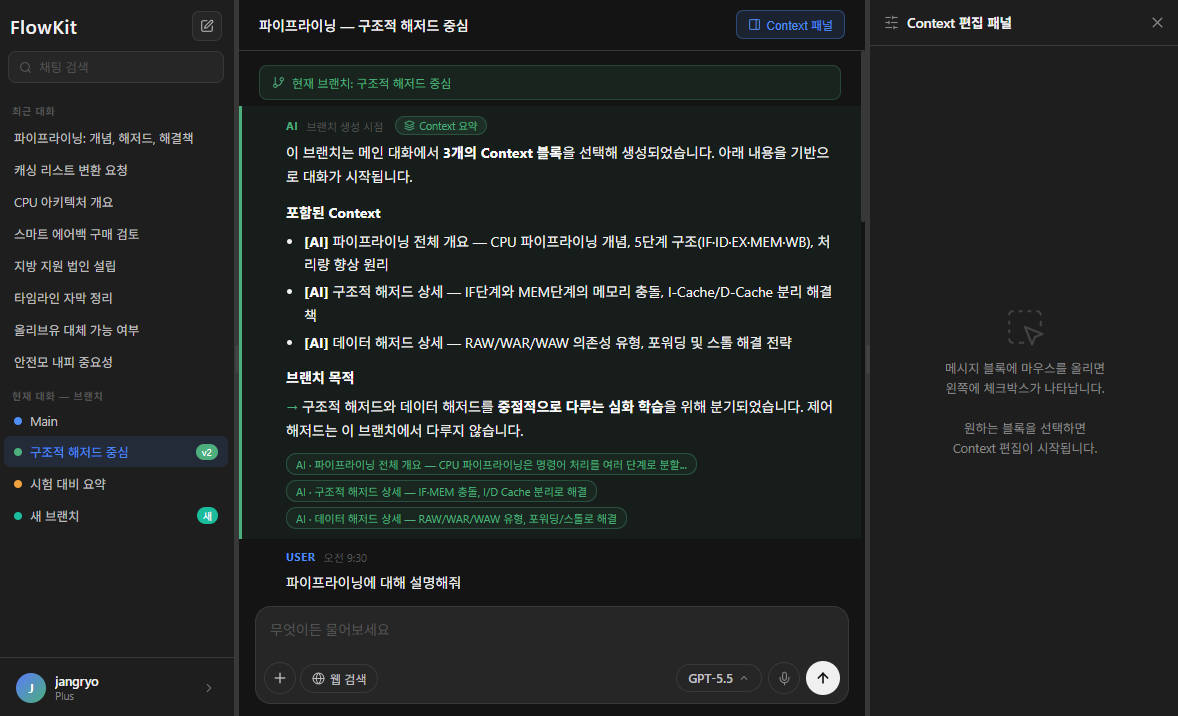
\includegraphics[width=\columnwidth]{images/그림4-2.png}
  \caption{브랜치 생성 결과 및 Context 요약 화면}
  \label{fig:fig4b}
\end{figure}

\subsection*{5. 시스템 구조 설계}

FlowKit의 시스템 구조는 Frontend, Backend, AI Context Processor, Database / Storage, Evaluation Logger로 나누어 설계하였다.

\begin{figure}[H]
  \centering
  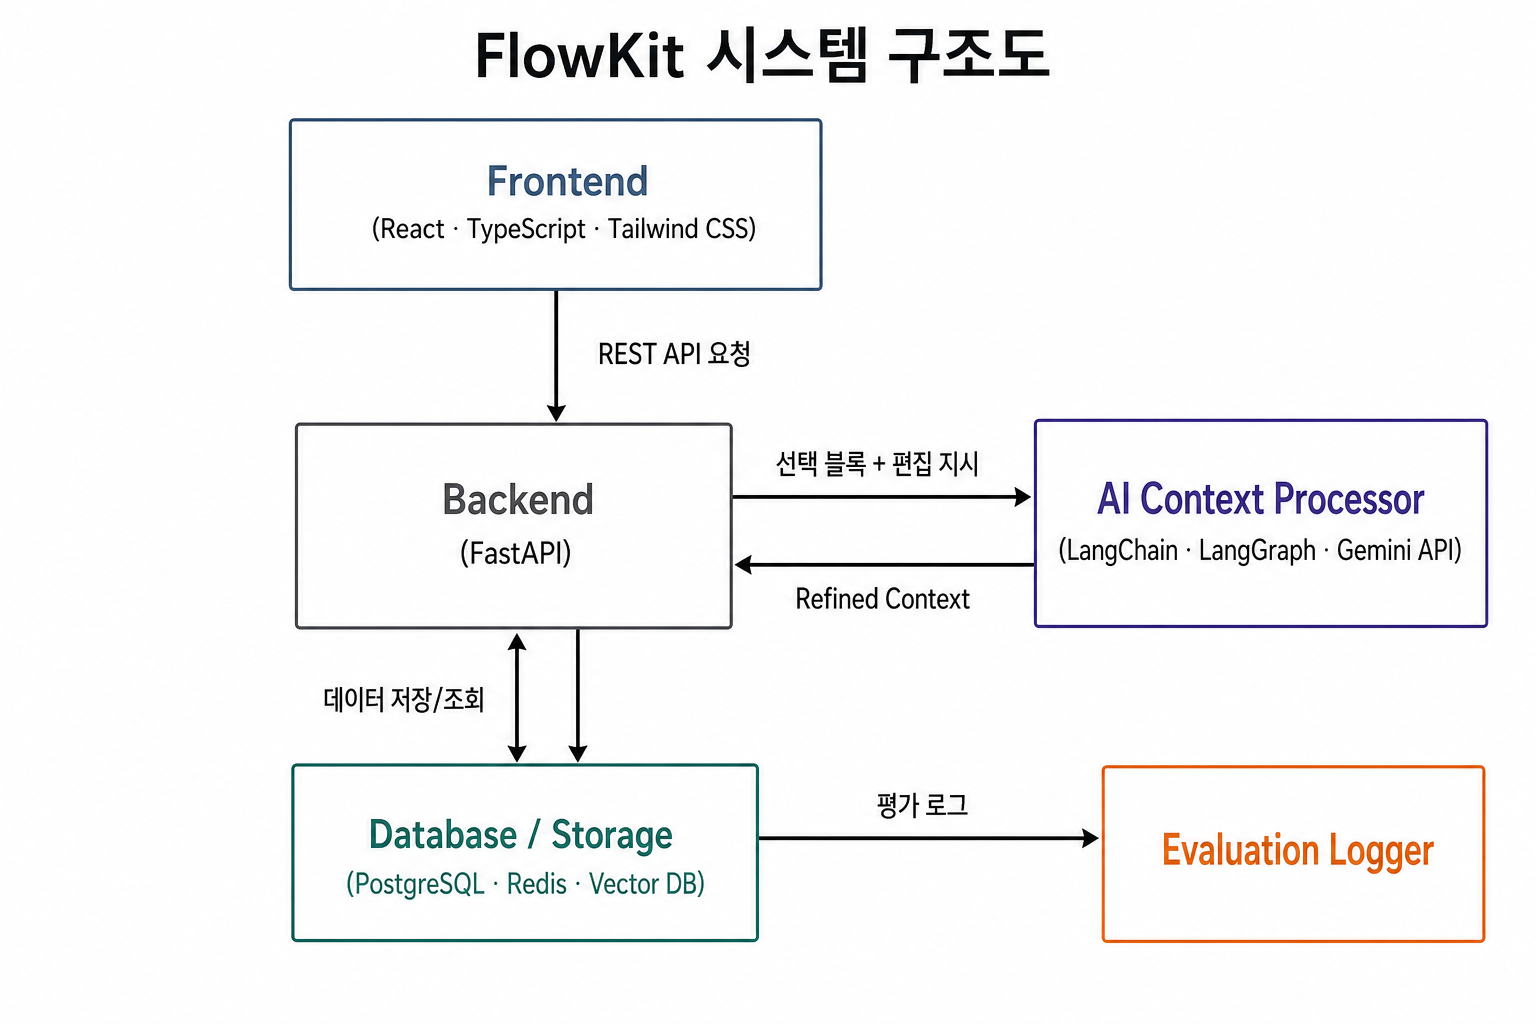
\includegraphics[width=\columnwidth]{images/figure5_system_architecture.png}
  \caption{FlowKit 시스템 구조도 — Frontend, Backend, AI Context Processor, Database / Storage, Evaluation Logger 간의 데이터 흐름 관계}
  \label{fig:fig5}
\end{figure}

\begin{table}[H]
\centering
\caption{FlowKit 시스템 모듈별 역할}
\label{tab:modules}
\small
\begin{tabularx}{\columnwidth}{@{} l X @{}}
\toprule
\textbf{모듈} & \textbf{역할} \\
\midrule
Frontend             & UI 표시 및 사용자 조작 처리 \\
Backend              & API 및 서비스 로직 처리 \\
AI Context Processor & Context 정제 및 prompt 구성 \\
Database / Storage   & 데이터 저장 \\
Evaluation Logger    & 평가 로그 수집 \\
\bottomrule
\end{tabularx}
\end{table}

기술 스택은 Frontend(React, TypeScript), Backend(FastAPI), AI Workflow(LangChain/LangGraph), Cache(Redis), Database(PostgreSQL), LLM API(Gemini / OpenAI)로 구성된다. 캡스톤디자인(2)에서는 FastAPI와 React를 중심으로 MVP를 구현하고, LangGraph, Redis 등은 핵심 기능 안정화 이후 단계적으로 적용한다.

\subsection*{6. Context 처리 흐름}

FlowKit의 Context 처리 흐름은 원본 대화 로그(Raw Conversation)와 활성 Context(Active Prompt)를 분리하는 방식으로 설계한다.

\begin{figure}[H]
  \centering
  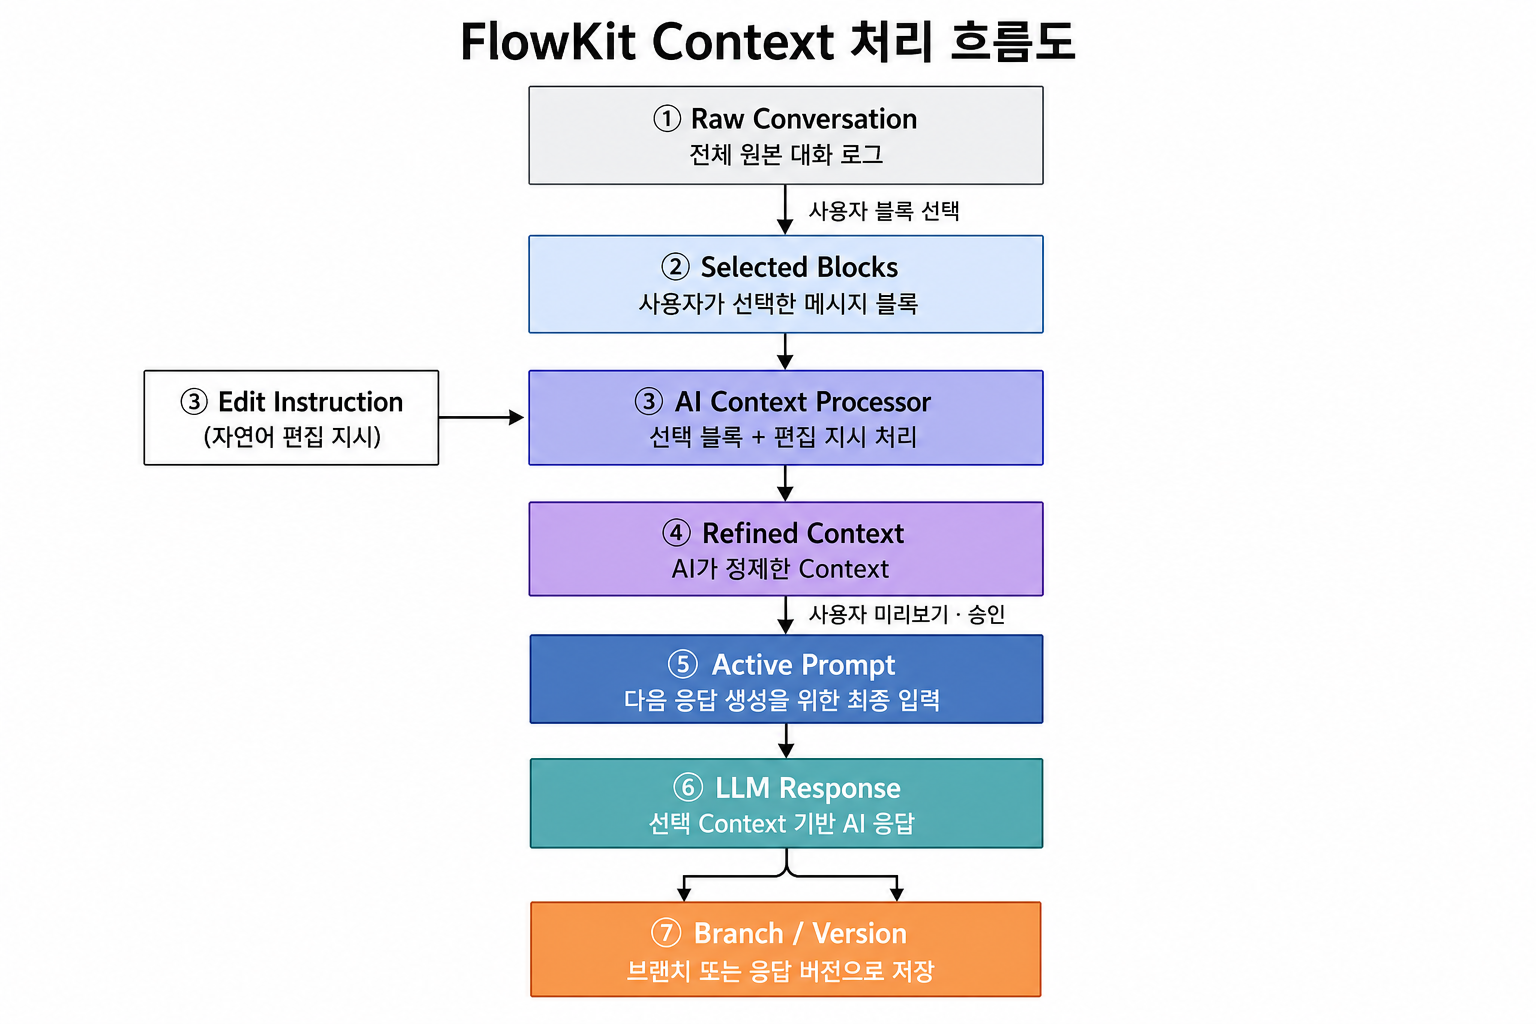
\includegraphics[width=\columnwidth]{images/figure6_context_flow.png}
  \caption{FlowKit Context 처리 흐름도 — Raw Conversation에서 Selected Blocks가 추출되고, AI Context Processor를 거쳐 Active Prompt로 구성되어 LLM Response가 생성되는 전체 흐름}
  \label{fig:fig6}
\end{figure}

사용자가 메시지 블록을 선택하면 해당 블록들은 Selected Blocks로 저장된다. 사용자의 자연어 지시와 함께 AI Context Processor로 전달되어 Refined Context가 생성되고, 사용자 승인 후 Active Prompt에 포함되어 LLM 응답 생성에 사용된다.

\begin{table}[H]
\centering
\caption{Context 처리 단계}
\label{tab:stages}
\small
\begin{tabularx}{\columnwidth}{@{} c l X @{}}
\toprule
\textbf{단계} & \textbf{데이터} & \textbf{설명} \\
\midrule
1 & Raw Conversation & 전체 원본 대화 로그 \\
2 & Selected Blocks  & 사용자가 선택한 메시지 블록 \\
3 & Edit Instruction & 사용자의 자연어 편집 지시 \\
4 & Refined Context  & AI가 정제한 Context \\
5 & Active Prompt    & 최종 LLM 입력 \\
6 & LLM Response     & 선택 Context 기반 AI 응답 \\
7 & Branch / Version & 브랜치 또는 응답 버전으로 저장 \\
\bottomrule
\end{tabularx}
\end{table}

\subsection*{7. 평가 계획}

캡스톤디자인(2)에서는 일반 선형 챗봇 방식과 FlowKit 방식을 비교하여 Context 관리 효과를 검증한다. 평가는 파일럿 테스트(5명)와 본 사용자 테스트(8\textasciitilde10명)로 나누어 수행한다.

\begin{table}[H]
\centering
\caption{정량 평가 지표 및 목표}
\label{tab:metrics}
\small
\begin{tabularx}{\columnwidth}{@{} X c @{}}
\toprule
\textbf{평가 항목} & \textbf{목표} \\
\midrule
토큰 절감률          & 평균 30\% 이상 \\
선택 Context 반영률  & 평균 80\% 이상 \\
불필요 Context 혼입률 & 평균 20\% 이하 \\
응답 초점성          & 평균 4.0점 이상 \\
브랜치 목적 일치도    & 평균 4.0점 이상 \\
태스크 완료율         & 80\% 이상 \\
\bottomrule
\end{tabularx}
\end{table}

사용자 평가는 5점 Likert 척도로 사용자 제어감, 맥락 이해 용이성, 사용 편의성, 결과 신뢰도, 재사용 의향을 측정한다.

\subsection*{8. 추진 일정}

캡스톤디자인(1)에서는 요구사항정의서 작성을 포함한 기획·설계를 완료하였다. 소프트웨어 설계서(FL·BL·AI 모듈별 기능 문서, API 명세, 아키텍처 설계)는 여름학기 내 완성을 목표로 작성이 진행 중이며, 설계서 완성 후 개발에 착수한다. 여름학기(7\textasciitilde8월)에는 소프트웨어 설계서 완성, 기능 통합 준비, 핵심 기능 구현을 수행하고, 캡스톤디자인(2)(9\textasciitilde12월)에서는 성능 비교, 사용자 테스트, 최종 정리를 진행한다.

\begin{table}[H]
\centering
\caption{캡스톤디자인(2) 추진 일정}
\label{tab:schedule}
\small
\begin{tabularx}{\columnwidth}{@{} c X @{}}
\toprule
\textbf{기간} & \textbf{주요 내용} \\
\midrule
9월       & AI Context 정제, 브랜치 기능 구현 \\
10월      & 성능 비교 및 정량 평가 \\
11월      & 사용자 테스트 및 피드백 수집 \\
11\textasciitilde12월 & 서비스 공개 검토 \\
12월      & 최종 보고서 작성 및 시연 준비 \\
\bottomrule
\end{tabularx}
\end{table}

% ─────────────────────────────────────────────────────────
\section*{Ⅳ. 결론}
% ─────────────────────────────────────────────────────────

\subsection*{1. 연구 요약}

본 연구에서는 기존 AI 챗봇의 선형적 Context 누적 구조가 가진 문제를 분석하고, 이를 해결하기 위한 사용자 주도형 Context 관리 서비스 FlowKit을 제안하였다. FlowKit은 대화를 메시지 블록 단위로 구조화하여, 사용자가 필요한 블록만 선택하고 자연어 지시로 Context를 정제한 뒤 후속 질문 또는 새로운 브랜치에 적용할 수 있도록 설계하였다.

캡스톤디자인(1)에서는 문제 정의, 선행연구 조사, UI/UX 프로토타입 설계, 시스템 구조 설계, 요구사항정의서 작성, 평가 계획 수립까지 전체 설계 기반을 완료하였다. 요구사항정의서에는 기능 요구사항 65개와 비기능 요구사항 19개를 수용 기준과 함께 정의하였으며, MVP 필수 요구사항 17개 항목을 확정하였다. 이를 통해 캡스톤디자인(2)에서는 별도의 기획 재정의 없이 MVP 구현과 사용자 검증에 집중할 수 있다.

\subsection*{2. 활용 분야}

FlowKit은 학습 및 시험 대비, 문서 작성 및 기획, 정보 요약 및 정리, 오류 수정 및 방향 전환 등 여러 턴에 걸친 장기 AI 대화 작업 전반에 활용될 수 있다.

\subsection*{3. 향후 확장 가능성}

기본 기능이 안정화된 이후에는 팀 협업 기능, Context 템플릿, 외부 문서 연동(RAG), 분석 대시보드, 제한적 웹 서비스 공개 등의 방향으로 확장할 수 있다. FlowKit은 긴 AI 대화에서 사용자가 필요한 맥락을 직접 선택하고 관리할 수 있도록 하는 HCI 기반 Context Engineering 서비스로서의 의의가 있다.

\subsection*{4. 연구의 한계}

본 연구는 설계 단계에서 도출된 몇 가지 내재적 한계를 지닌다. 첫째, 메시지 블록을 수동으로 선택하는 과정 자체가 인지 부하를 높일 수 있다. 특히 단발성 대화나 짧은 작업에서는 Context 정제 과정이 일반 챗봇 대비 오버헤드로 작용할 수 있으며, 이는 대화 복잡도에 따른 UI 적응 설계를 통해 완화할 수 있을 것으로 기대된다. 둘째, 평가 계획의 8\textasciitilde10명 규모 사용자 테스트는 예비적 검증 수준에 해당하므로, 통계적 유의성 확보를 위한 대규모 후속 연구가 필요하다. 셋째, 현재 설계는 텍스트 기반 대화를 전제하므로, 코드 편집이나 멀티모달 입력 등 특수 용도 대화에 대한 확장성 검토가 추가로 요구된다. 이러한 한계들은 후속 구현 및 사용자 검증을 통해 실증적으로 확인하고 보완되어야 할 사항이다.

\end{multicols}

% ============================================================
%  참고문헌 (1단, 전체 폭)
% ============================================================
\hrule\vspace{6pt}
\begin{thebibliography}{10}
\small

\bibitem{li2026}
H.\ Li, Q.\ Zhang, P.\ Wang, and Z.\ Lu,
``Mixed-Initiative Context: Structuring and Managing Context for Human-AI Collaboration,''
\textit{arXiv:2604.07121}, 2026.

\bibitem{nanjundappa2025}
B.\ C.\ Nanjundappa and S.\ Maaheshwari,
``Context Branching for LLM Conversations: A Version Control Approach to Exploratory Programming,''
\textit{arXiv:2512.13914}, 2025.

\bibitem{liu2024}
N.\ F.\ Liu, K.\ Lin, J.\ Hewitt, A.\ Paranjape, M.\ Bevilacqua, F.\ Petroni, and P.\ Liang,
``Lost in the Middle: How Language Models Use Long Contexts,''
\textit{Transactions of the Association for Computational Linguistics}, vol.\ 12, pp.\ 157--173, 2024.
DOI: \href{https://doi.org/10.1162/tacl_a_00638}{10.1162/tacl\_a\_00638}.

\bibitem{laban2025}
P.\ Laban, H.\ Hayashi, Y.\ Zhou, and J.\ Neville,
``LLMs Get Lost In Multi-Turn Conversation,''
\textit{arXiv:2505.06120}, 2025.

\bibitem{packer2023}
C.\ Packer, S.\ Wooders, K.\ Lin, V.\ Fang, S.\ G.\ Patil, I.\ Stoica, and J.\ E.\ Gonzalez,
``MemGPT: Towards LLMs as Operating Systems,''
\textit{arXiv:2310.08560}, 2023.

\bibitem{tso2026}
J.\ Tso, P.\ Schmittou, Q.\ Huynh, and J.\ Hutchins,
``ConstraintBench: Benchmarking LLM Constraint Reasoning on Direct Optimization,''
\textit{arXiv:2602.22465}, 2026.

\end{thebibliography}

\end{document}
